\scanpage{115}
\deleted{1) \(\unsure{\dim X=n=2}\)}

\uline{Ex.}\quad \(n=2\)

\textcircled{1}
\diagram{\begin{array}{lll}
A_r^0(X)\ \unsure{\text{---}|\longrightarrow}\ A_r^0(Y)&\text{bijectif exc }p&\text{OK}\\
A_r^1(X)^\tau\longrightarrow A_r^1(Y)^\tau&\text{injectif exc. }p&\text{OK}
\end{array}}

\textcircled{2}
\diagram{\begin{array}{lll}
A_0^r(Y)\ \unsure{\text{---}|\longrightarrow}\ A_0^r(X)&\text{surjectif exc. }p&\text{OK}\\
A_0^r(Y)^\tau\ \unsure{\text{---}|\longrightarrow}\ A_0^r(X)^\tau&\text{----}&\text{OK}\\
\begin{array}{ccc}A_0^a(Y)&\longrightarrow&A_0^a(X)\\\Vert&&\Vert\\Z&&Z\end{array}&\text{bijectif exc. }p&\text{OK}
\end{array}}
\margin{du moins si équiv. rat. des 0-cycles = équiv. d'Albanese\ldots}

\textcircled{3}
\diagram{\begin{array}{lll}
\left.\begin{array}{ccc}A_a^0(X)&\xrightarrow{E^2}&A_a^2(X)\\\Vert&&\Vert\\Z&&Z\\A_a^1(X)&\overset{E^0=\mathrm{id}}{\unsure{\text{---}|\longrightarrow}}&A_a^1(X)\end{array}\right\}&\text{bijectif mod grp finis}&\text{OK.}\\[6pt]
\left.\begin{array}{ccc}A_r^0(X)^\tau&\longrightarrow&A_{\unsure{a|r}}^2(X)\\\Vert&&\Vert\\0&&0\\A_r^1(X)^\tau&\xrightarrow{\mathrm{id}}&A_r^1(X)^\tau\end{array}\right\}&\text{bij. mod grp finis}&\text{OK.}
\end{array}}

\textcircled{2'}\quad \(A_0^r(U)=0\)
\margin{O.K. si équivalence rationnelle = équiv. d'Albanese}

\uline{Ex.}\quad \(n=3\)

\textcircled{1}
\diagram{\begin{array}{lll}
A_r^0(X)\ \unsure{\text{---}|\longrightarrow}\ A_r^0(Y)&\text{bij. exc. }p&\text{O.K.}\\
A_r^1(X)\ \unsure{\text{---}|\longrightarrow}\ A_r^1(Y)&\text{injectif exc }p.&\text{O.K.}\\
A_r^1(X)^\tau\ \unsure{\text{---}|\longrightarrow}\ A_r^1(Y)^\tau&\text{bijectif exc }p&\text{O.K.}
\end{array}}

\textcircled{2}
\diagram{\begin{array}{lll}
A_0^r(Y)\ \unsure{\text{---}|\longrightarrow}\ A_0^r(X)&\text{bijectif exc. }p&\text{O.K.}\\
A_1^a(Y)\longrightarrow A_1^a(X)&\text{surjectif exc. }p&\textcircled{?}
\end{array}}
\margin{si équiv. rat. = équiv. Alb.}

\textcircled{3}
\diagram{\begin{array}{lll}
\begin{array}{ccc}A_a^0(X)&\overset{E^3}{\unsure{\text{---}|\longrightarrow}}&A_a^3(X)\\\simeq Z&&\simeq Z\end{array}&\text{bijectif mod grp finis}&\text{OK.}\\
A_a^1(X)\overset{E^1}{\unsure{\text{---}|\longrightarrow}}A_a^2(X)&\deleted{\text{\unsure{bijectif|surjectif}}}&\\
&\text{bijectif mod grp finis}&
\end{array}}
\figure{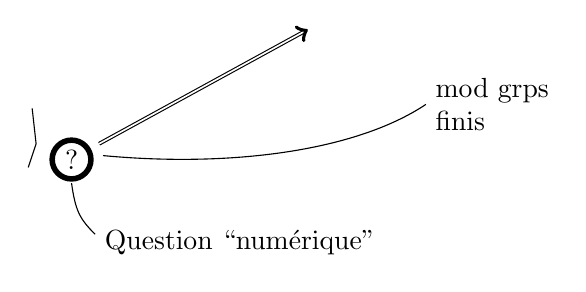
\begin{tikzpicture}[x=1cm,y=1cm]
\node[draw,circle,line width=2pt,inner sep=2pt](q) at(0,0){?};
\draw[->,double] (.35,.2)--(3,1.65);
\draw(0,-.3)..controls(.05,-.65)and(.1,-.75)..(.3,-.95);
\node[anchor=west] at(.3,-1.05){Question ``numérique''};
\draw(.4,.05)..controls(2,-.1)and(3.6,.1)..(4.5,.7);
\node[anchor=west,align=left] at(4.5,.7){\unsure{mod} \unsure{grps}\\finis};
\draw(-.5,.65)--(-.45,.2)--(-.55,-.1);
\end{tikzpicture}}
\margin{114}
